\documentclass{article}%book,report,letter
\usepackage{booktabs}
\usepackage{ctex}
\usepackage{graphicx}
\usepackage{amsmath}
\usepackage{amsthm}
\usepackage{float}
\graphicspath{{figures/}}
\title{学习报告}
\author{姜钦瀚}
\newtheorem{definition}{\bf 定义}[section]
\newtheorem{pro}{\bf 命题}[section]
\newtheorem{thm}{\bf 定理}[section]
\newtheorem{lemma}{\bf 引理}[section]
\begin{document}
	\maketitle
考虑如下的随机微分方程
\begin{equation}
d X_{t}=a\left(t, X_{t}\right) d t+b\left(t, X_{t}\right) d W_{t},t_0\leq t \leq T,\\
X_{t_0}=X_0
\end{equation}
给定时间划分$t_{0}=\tau_{0}<\tau_{1}<\cdots<\tau_{n}<\cdots<\tau_{N}=T$,记$\Delta_n=\tau_{n+1}-\tau_{n}$,$\delta=max\Delta_n$。
\section{定义}
\begin{definition}
称格式$Y_\delta$在T处强收敛于X如果	
\begin{equation}
\lim _{\delta \downarrow 0} E\left(\left|X_{T}-Y^{\delta}(T)\right|\right)=0
\end{equation}
\end{definition}
\section{strong scheme}
$\mathcal{A}=\Lambda_{k}:=\{\alpha ; \quad \alpha \in \mathcal{M}, l(\alpha)+n(\alpha) \leq 2 k$
or $\left.l(\alpha)=n(\alpha)=k+\frac{1}{2}\right\}$ 
,K阶强格式为
\begin{equation}X^{n+1}=\sum_{\alpha \in \Lambda_{k}} I_{\alpha}\left[f_{\alpha}\left(t_{n}, X^{n}\right)\right]_{t_{n}, t_{n+1}}=\sum_{\alpha \in \Lambda_{k}} f_{\alpha}\left(t_{n}, X^{n}\right) I_{\alpha, t_{n}, t_{n+1}}\end{equation}
\section{Euler格式}
Euler格式是强0.5阶格式定义$\mathcal{A}$为\begin{equation}\mathcal{A}=\{\phi,(0),(1)\}=\Lambda_{0.5}\end{equation}
由上面定义可知设Brown运动有m个分量,k维的Euler格式为
\begin{equation}
Y_{n+1}^{k}=Y_{n}^{k}+a^{k} \Delta+\sum_{j=1}^{m} b^{k, j} \Delta W^{j}
\end{equation}
\subsection{数值模拟}
考虑如下的线性随机微分方程
\begin{equation}d X(t)=\lambda X(t) d t+\mu X(t) d W(t), \quad X_{t_0}=X_{0}\end{equation}
其真解为
\begin{equation}X(t)=X_{t_0} \exp \left(\left(\lambda-\frac{1}{2} \mu^{2}\right) t+\mu W(t)\right)\end{equation}
取区间为$[0,1]$将区间均匀剖分,$\delta=10^{-5}$,模拟出真解的情况,然后取$\delta=0.1$应用欧拉格式,数值模拟结果如下
\begin{figure}[h]
	\centering
	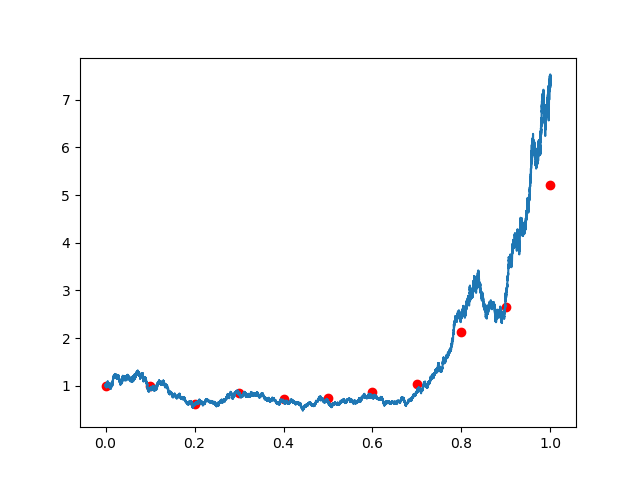
\includegraphics[width=6cm,height=4cm]{Figure_1.png}\\
	\centering	
\end{figure}
分别取$\delta=10^{-i},i=\{0,1,2,3,4\}$,各重复实验1000次,取$T=1$处的误差,并求平均值来模拟
$E\left(\left|X_{T}-Y^{\delta}(T)\right|\right)$
结果见下面表格
\begin{table}[htbp]
	\centering
	\caption{误差}
	\begin{tabular}{ccccc}
		\toprule  % 顶部线
		1&2&3&4&5 \\ 
		\midrule  % 中部线
		4.26748204&1.481642574&0.45718003&0.13571932&0.03757269 \\
		\bottomrule  % 底部线
	\end{tabular}
\end{table}
\section{Milstein格式}
Milstein格式是强1阶格式,\begin{equation}\mathcal{A}=\{\phi,(0),(1),(1,1)\}=\Lambda_{1}\end{equation}。代入$Ito-Taylor$展开得
\begin{equation}\begin{aligned}
X^{n+1}=& \sum_{\alpha \in \Lambda_{1}} I_{\alpha}\left[f_{\alpha}\left(t_{n}, X^{n}\right)\right]_{t_{n}, t_{n+1}}=\sum_{\alpha \in \Lambda_{1}} f_{\alpha}\left(t_{n}, X^{n}\right) I_{\alpha, \text {tn}, t_{n+1}} \\
=& f_{\phi}\left(t_{n}, X^{n}\right) I_{\phi, t_{n}, t_{n+1}}+f_{(0)}\left(t_{n}, X^{n}\right) I_{(0), t_{n}, t_{n+1}}+f_{(1)}\left(t_{n}, X^{n}\right) I_{(1), t_{n}, t_{n+1}} \\
&+f_{(1,1)}\left(t_{n}, X^{n}\right) I_{(1,1), t_{n}, t_{n+1}} \\
=& X^{n}+a\left(t_{n}, X^{n}\right) \Delta t_{n}+b\left(t_{n}, X^{n}\right) \Delta W_{t n}+f_{(1,1)}\left(t_{n}, X^{n}\right) \int_{t_{n}}^{t_{n+1}} \int_{t_{n}}^{s} d W_{\tau}^{1} d W_{s}^{1}
\end{aligned}\end{equation}
\subsection{数值模拟}
考虑如下的线性随机微分方程
\begin{equation}d X(t)=\lambda X(t) d t+\mu X(t) d W(t), \quad X_{t_0}=X_{0}\end{equation}
其真解为
\begin{equation}X(t)=X_{t_0} \exp \left(\left(\lambda-\frac{1}{2} \mu^{2}\right) t+\mu W(t)\right)\end{equation}
取区间为$[0,1]$将区间均匀剖分,$\delta=10^{-5}$,模拟出真解的情况,然后取$\delta=0.1$应用Milstein格式,数值模拟结果如下
\begin{figure}[h]
	\centering
	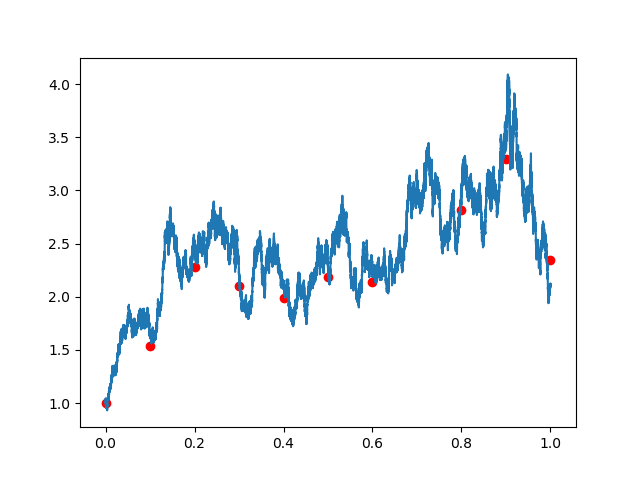
\includegraphics[width=6cm,height=4cm]{Figure_2.png}\\
	\centering	
\end{figure}
分别取$\delta=10^{-i},i=\{0,1,2,3,4\}$,各重复实验1000次,取$T=1$处的误差,并求平均值来模拟
$E\left(\left|X_{T}-Y^{\delta}(T)\right|\right)$
结果见下面表格
\begin{table}[htbp]
	\centering
	\caption{误差变化}
	\begin{tabular}{ccccc}
		\toprule  % 顶部线
		1&2&3&4&5 \\ 
		\midrule  % 中部线
		4.576793014&1.481642574&0.16355771&0.01529428&0.00159989 \\
		\bottomrule  % 底部线
	\end{tabular}
\end{table}
\section{强1.5阶格式}
\begin{equation}\mathcal{A}=\left\{\begin{array}{cccc}
\emptyset, & (0), & (1), & (1,1)\\
(0,0), & (1,0), & (0,1),& (1,1,1)\\
\end{array}\right\}=\Lambda_{1,5}\end{equation}
$\alpha=(0,0)$对应
\begin{equation}\begin{aligned}
f_{(0,0)} &=L^{0} L^{0} f=L^{0} a \\
&=\frac{\partial a}{\partial t}+a \frac{\partial a}{\partial x}+\frac{1}{2} b^{2} \frac{\partial^{2} a}{\partial x^{2}} \\
I_{(0,0), t_{n}, t_{n+1}} &=\int_{t_{n}}^{t_{n+1}} \int_{t_{n}}^{t} d s d t=\frac{1}{2} \Delta t_{n}
\end{aligned}\end{equation}
$\alpha=(1,0)$对应
\begin{equation}\begin{aligned}
f_{(1,0)} &=L^{1} L^{0} f=L^{1} a=b \frac{\partial a}{\partial x} \\
I_{(1,0), t_{n}, t_{n+1}} &=\int_{t_{n}}^{t_{n+1}} \int_{t_{n}}^{t} d W_{s} d t=\Delta Z_{n}
\end{aligned}\end{equation}
$\alpha=(0,1)$对应
\begin{equation}\begin{aligned}
f_{(0,1)} &=L^{0} L^{1} f=L^{0} b \\
&=\frac{\partial b}{\partial t}+a \frac{\partial b}{\partial x}+\frac{1}{2} b^{2} \frac{\partial^{2} b}{\partial x^{2}} \\
I_{(0,1)}, t_{n}, t_{n+1} &=\int^{t_{n+1}} \int_{t}^{t} d s d W_{t}=\overline{\Delta Z_{n}}
\end{aligned}\end{equation}
$\alpha=(1,1,1)$对应
\begin{equation}\begin{aligned}
f_{(1,1,1)} &=L^{1} L^{1} L^{1} f=L^{1} L^{1} b=L^{1}\left(b \frac{\partial b}{\partial x}\right) \\
&=b \frac{\partial}{\partial x}\left(b \frac{\partial b}{\partial x}\right)=b\left(\frac{\partial b}{\partial x}\right)^{2}+b^{2} \frac{\partial^{2} b}{\partial x^{2}} \\
&=\int_{t n}^{t_{n+1}} \int_{t_{n}}^{t} \int_{t_{n}}^{s} d W_{r} d W_{s} d W_{t} \\
I_{(1,1,1)} t_{n}, t_{n+1}&=\frac{1}{2}\left(\frac{1}{3}\left(\Delta W_{t_{n}}\right)^{2}-\Delta t_{n}\right) \Delta W_{t_{n}}
\end{aligned}\end{equation}
\end{document}